\documentclass[a4paper,12pt]{article}
\usepackage[hidelinks]{hyperref}
\usepackage{graphicx}
\usepackage{float}
\usepackage{caption}

%% Title Page 
\title{\Huge Functional Requirements Document Specification \\ 
	 Project: \\ 
	Cafeteria Management System: Resolve}
\author{
         \underline{T-RISE}\\
          Rendani Dau (13381467) \\
	Elana Kuun (12029522) \\
	Semaka Malapane (13081129) \\
	Antonia Michael (13014171) \\
	Isabel Nel (13070305)\\ \\
	https://github.com/toniamichael94/MainProjectCOS301}

\date{\today}
 
%\documentclass[12pt]{article}

\begin{document}
\maketitle
\break

%% Make table of contents
\tableofcontents
\break

%%now begin document

%%---------------------------------  INTRODUCTION -------------------------------------------
\section{Introduction}
This document contains the functional requirements specification, architecture requirements and testing for the Resolve Cafeteria Management System that will be created for Software Engineering (COS 301) at the University of Pretoria 2015, by the group T-RISE. In this document we will thoroughly discuss and layout the project's functional requirements to provide a clear view of the system as a whole. An agile approach is being followed, hence the main use cases that this document will be focussing on are placing orders and managing a user profile. These will be explored in quite some detail.  The agile method involves an interactive and incremental method of managing and designing the system. 
%% ------------------------------ VISION ------------------------------------------------------
\section{Vision}
The vision of this project is to implement a flexible, pluggable, fully functional software application that will be maintainable, with detailed supporting documentation and an instruction manual for the Cafeteria Management System. This system will assist in managing the cafeteria's inventory/stock, executing orders from the cafeteria, generating bills and sending these to the appropriate parties and facilitating payments for access cards (or the use of unique access card numbers). 

%%---------------------------------- BACKGROUND -----------------------------------------
\section{Background}
As specified in the project proposal document from Resolve - the cafeteria is currently cash only and does not accept bank cards or electronic payments. This makes it inconvenient for employees as they have to carry around cash if they want to purchase anything from the cafeteria. Hence, this is equivalent to purchasing from an external food outlet where they can also pay with their preferred method of payment. The employees have to hence use up fuel and time and lastly this does not bring in the maximum amount of income to the cafeteria, hindering its growth and improvement.\\

Resolve is therefore looking for a means to accept payments from employees for the canteen using their employee access cards or access card numbers, with an amount being deducted from their salary at the end of the month.\\

Resolve proposed the Cafeteria Management System to assist with this problem.
After our first meeting with the client, they brought to our attention that at times the cafeteria does not even have enough stock to provide some of the menu items, thus the managing of inventory or stock will also be part of the system. The system will also predict what inventory/stock needs to be bought for the next week in order to avoid such a problem. At the end of each month, the bill for the month will be sent to either payroll or to the employee. This option is configurable from the user's profile. The employee can also set a spending limit for each month for control purposes. The system will have its own maximum, such that users cannot set a limit that exeeds this. 
 
%%--------------------------------------- FUNCTIONAL REQUIREMENTS--------------------------------
\section{Functional Requirements and Aplication Design}
In this section we will discuss the functional requirements. \\

%% ---------------USE CASES -------------------
\subsection{Use Cases }
Below is a list of all the use cases we have identified:

\begin{itemize}

\item  Login
\item Register
\item Manage Profile
\item Place Order
\item Notify
\item Manage Inventory
\item Report

\end{itemize}


%% ---------------USE CASE PRIORITIZATION -------------------
\subsection{Use Case Prioritization}
Below the use cases mentioned above will be catagorized as critical, important or nice to have.

\begin{itemize}

\subsubsection{Critical}
\item Login \\
This is a critical use case due to the fact that you cannot send through any order if you are not logged in. In such a case you will only be able to view the menu. 
 
\item Register \\
This is a critical use case because you can not log into the system if you have not been registered on the system. Furthermore, if you are not logged in , you can not place orders.

\item Place Order\\
This is critical due to the fact that the main functionality of the system revolves around the ability to place orders at the cafeteria as well as other activities relating to that. 

\subsubsection{Important}
\item Manage Profile \\
This use case is considered important because the user must be able edit their profile by resetting their personal spending limits and changing their email and passwords. The user must also be able to view his/her account history and current bill. It is crucial that the user is able to configure spending limits according to own preferences as well as keep track of monthly purchases.

\item Manage Inventory \\
This use case is considered important since this deals with incrementing stock that has been added and decrementing stock when it is purchased or expired. It also deals with the cafeteria manager marking orders as completed.

\item Reporting \\ 
This use case is considered important because users must be able to print a billing report and users must be able to send billing reports to Pay-Roll to have the amount spent per month deducted from their salaries. A history of all the orders that have taken place on the system can also be printed. 

\subsubsection{Nice to have}
\item Notify \\
This is classified as nice to have as it includes notifying a user when their order is ready for collection as well as other notifications such as notifying the casher or cafeteria manager that they are low on certain inventory.  The system is not dependant on this functionality.

\end{itemize}

%%--------------- USE CASE/SERVICE CONTRACTS --------------
\subsection{Use Case/Service Contracts}

\begin{figure}[H]
  \centering
    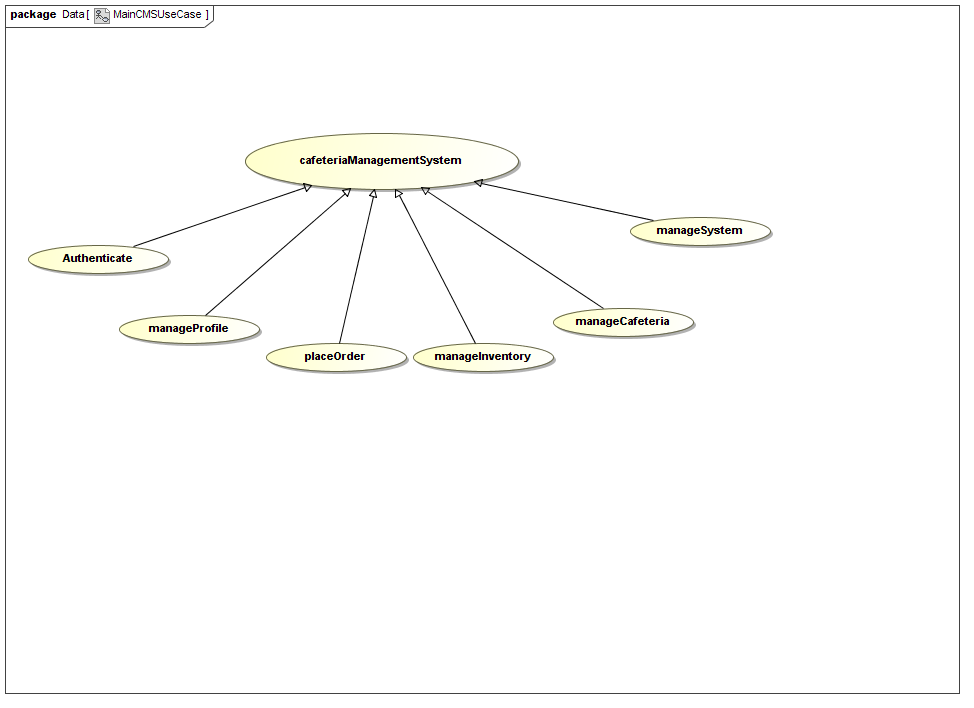
\includegraphics[width=1.0\textwidth]{images/CMSUseCase.png}
    \caption{Cafeteria Management System Use Case} 
\end{figure}

\begin{figure}[H]
  \centering
    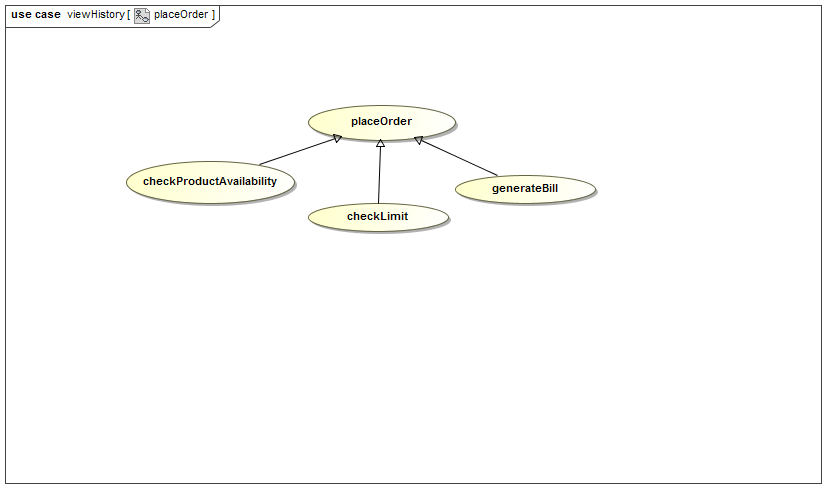
\includegraphics[width=1.0\textwidth]{images/placeOrder.png}
    \caption{Place Order Use Case} 
\end{figure}

\begin{figure}[H]
  \centering
    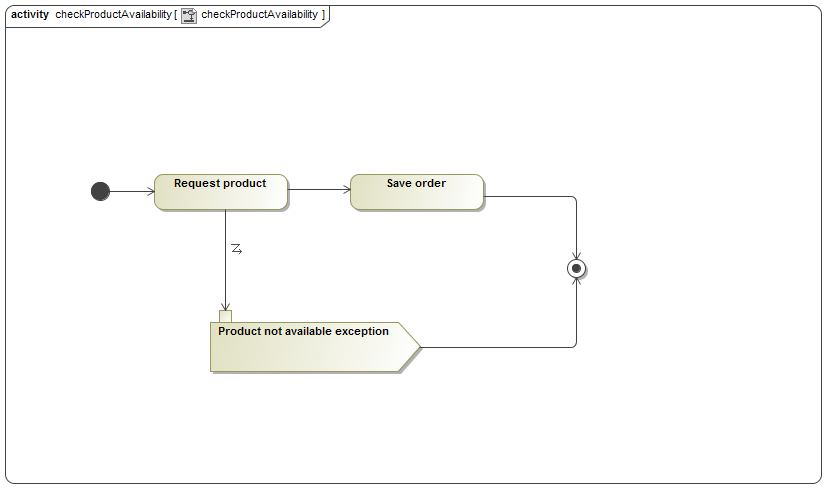
\includegraphics[width=1.0\textwidth]{images/checkProductAvailability.png}
    \caption{checkProductAvailability activity diagram} 
\end{figure}

\begin{figure}[H]
	\centering
	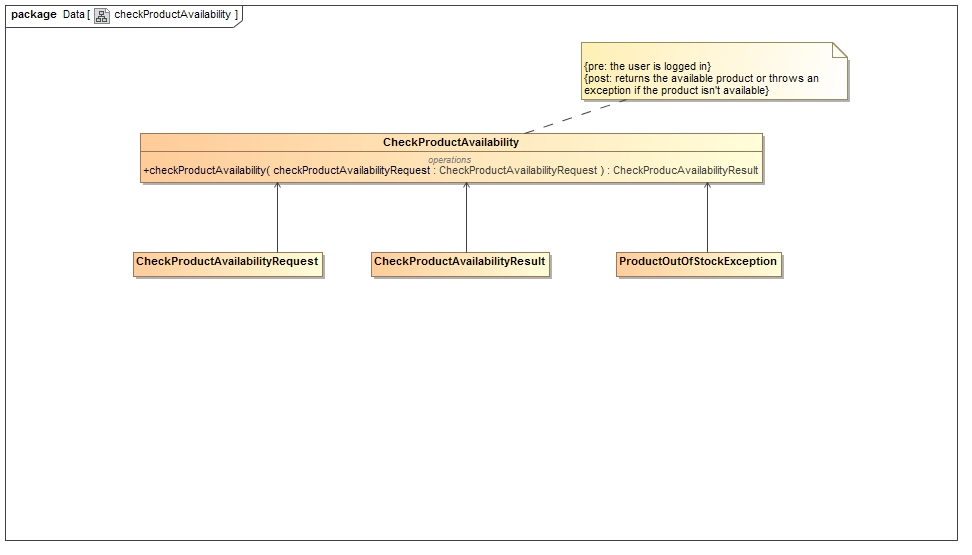
\includegraphics[width=1.0\textwidth]{images/checkProductAvailabilitySC.jpg}
	\caption{checkProductAvailability service contract}
\end{figure}

\begin{figure}[H]
  \centering
    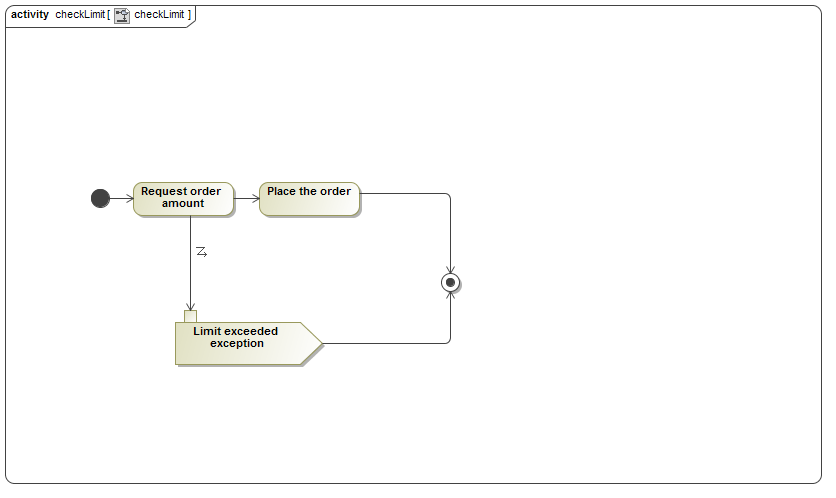
\includegraphics[width=1.0\textwidth]{images/checkLimit.png}
    \caption{checkLimit activity diagram} 
\end{figure}

\begin{figure}[H]
	\centering
	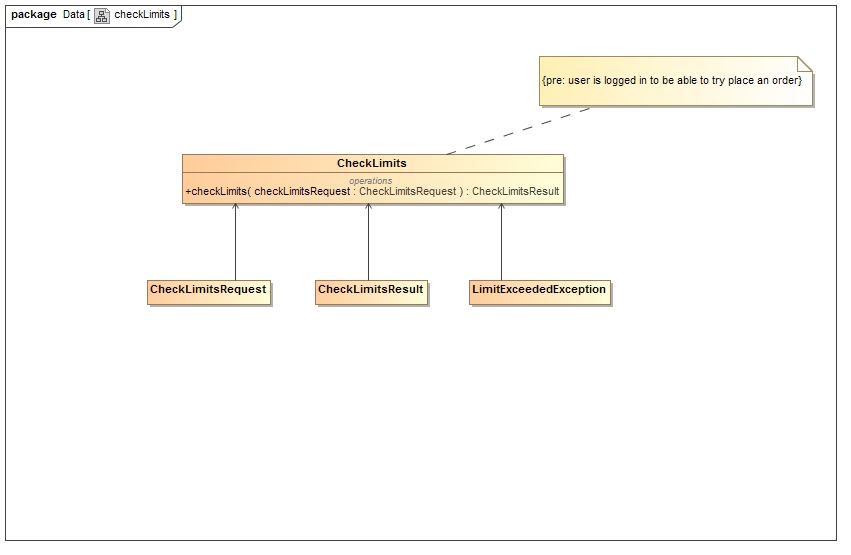
\includegraphics[width=1.0\textwidth]{images/checkLimitsSC.jpg}
	\caption{checkLimit service contract}
\end{figure}

\begin{figure}[H]
  \centering
    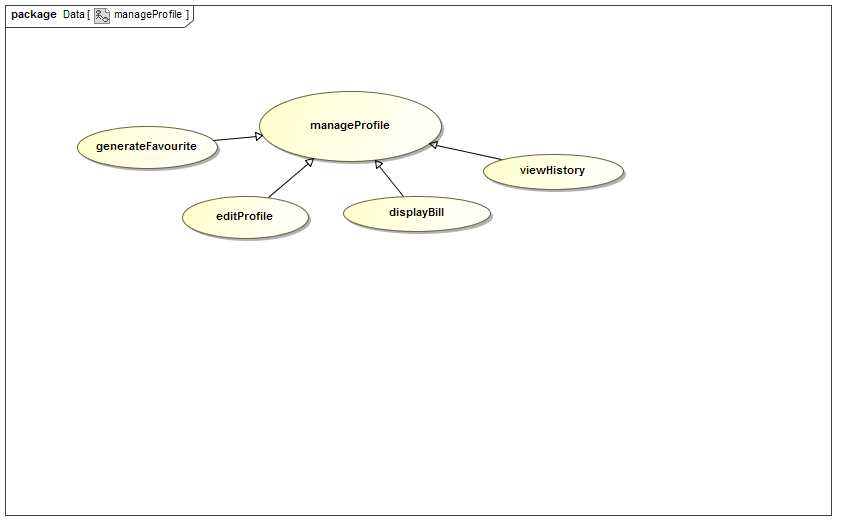
\includegraphics[width=1.0\textwidth]{images/manageProfile.png}
    \caption{manage profile use case} 
\end{figure}

\begin{figure}[H]
  \centering
    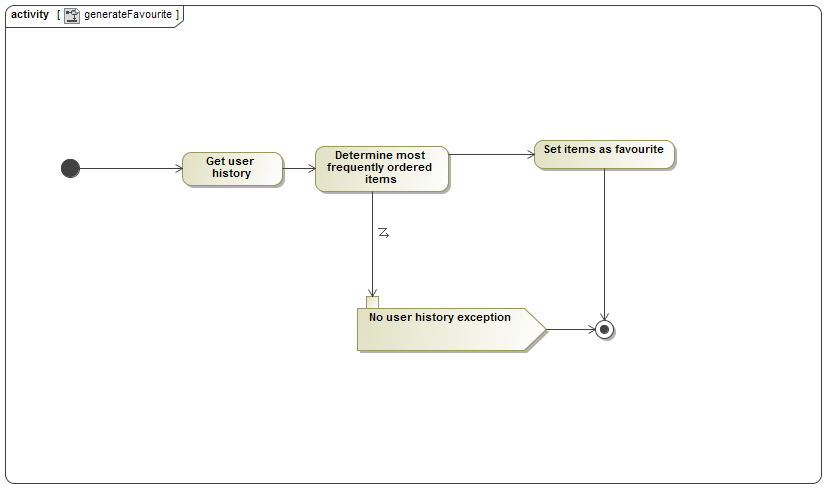
\includegraphics[width=1.0\textwidth]{images/generateFavourite.png}
    \caption{viewFavourite activity diagram} 
\end{figure}

\begin{figure}[H]
	\centering
	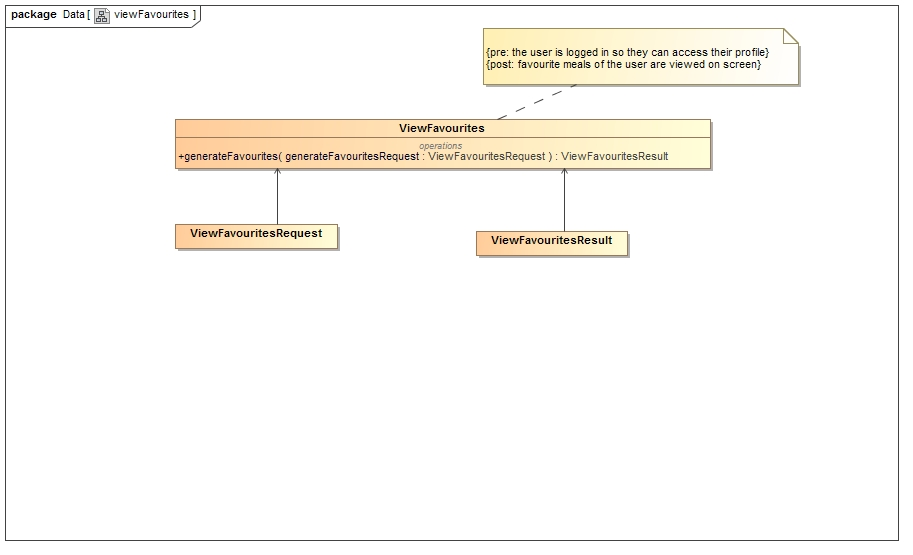
\includegraphics[width=1.0\textwidth]{images/viewFavouritesSC.jpg}
	\caption{viewFavourite service contract}
\end{figure}

\begin{figure}[H]
  \centering
    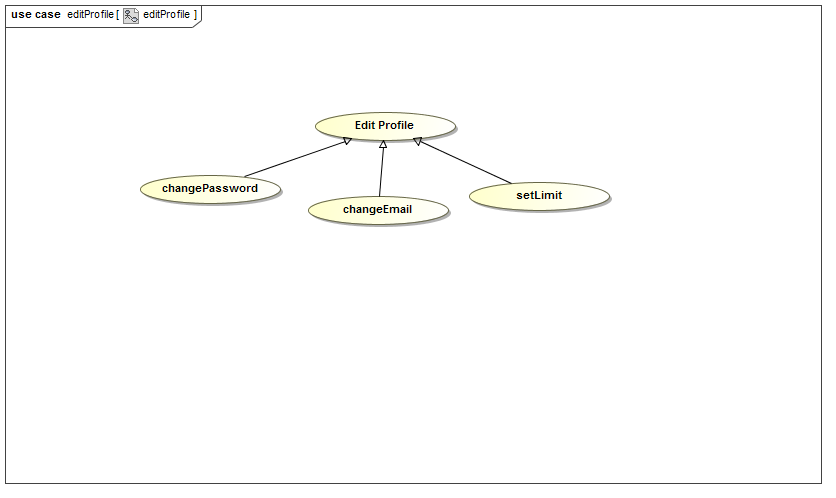
\includegraphics[width=1.0\textwidth]{images/editProfile.png}
    \caption{edit profile Use Case} 
\end{figure}

\begin{figure}[H]
  \centering
    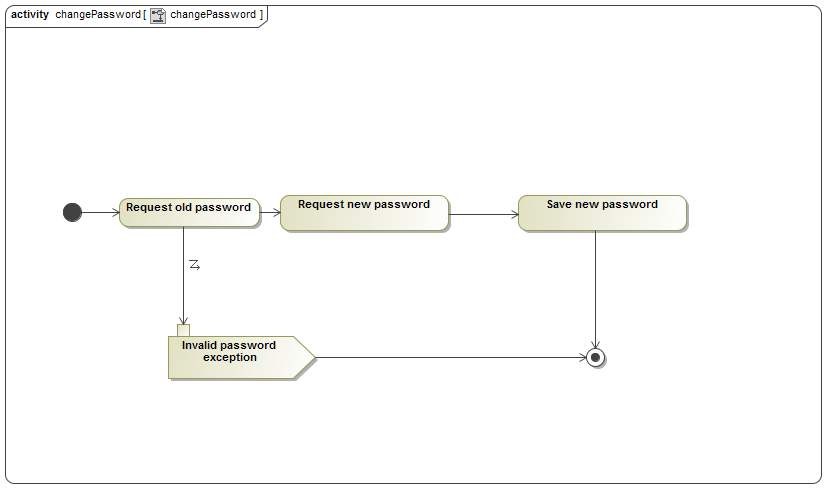
\includegraphics[width=1.0\textwidth]{images/changePassword.png}
    \caption{changePassword activity diagram} 
\end{figure}
	
\begin{figure}[H]
	\centering
	\includegraphics[width=1.0\textwidth]{images/changePasswordSC.jpg}
	\caption{changePassword service contract}
\end{figure}

\begin{figure}[H]
  \centering
    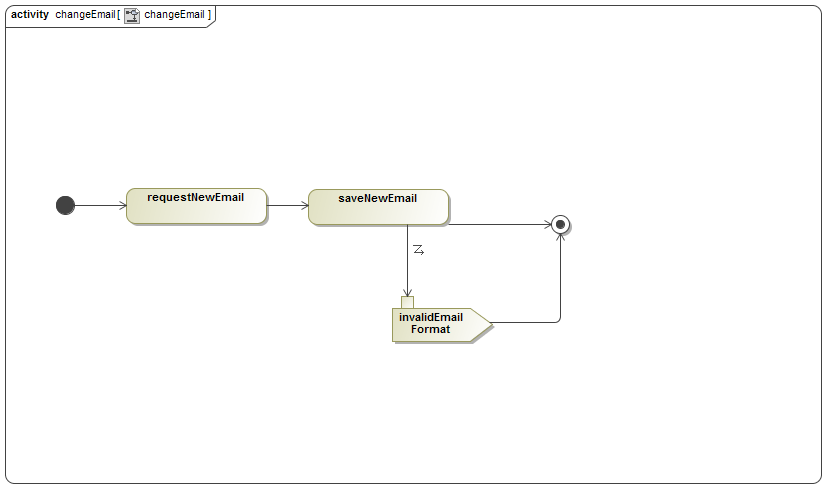
\includegraphics[width=1.0\textwidth]{images/changeEmail.png} 
    \caption{changeEmail activity diagram}
\end{figure}
	
\begin{figure}[H]
	\centering
	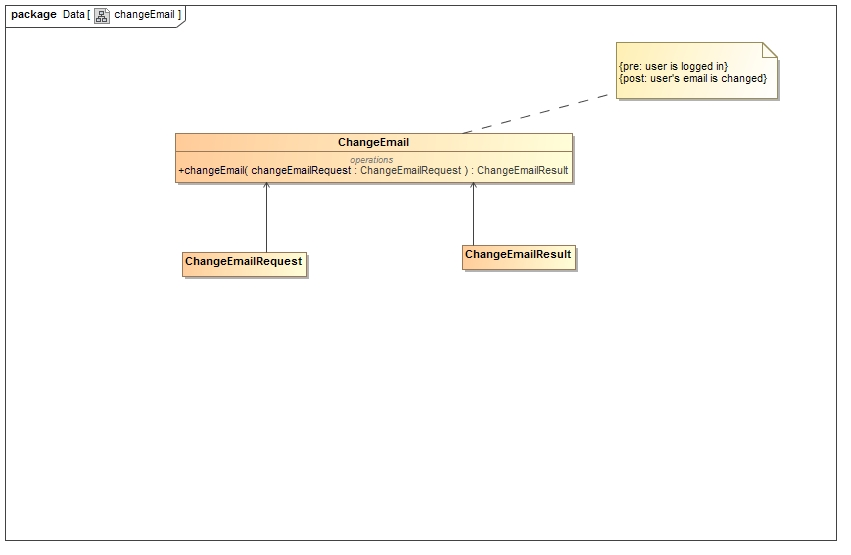
\includegraphics[width=1.0\textwidth]{images/changeEmailSC.jpg}
	\caption{changeEmail service contract}
\end{figure}

\begin{figure}[H]
  \centering
    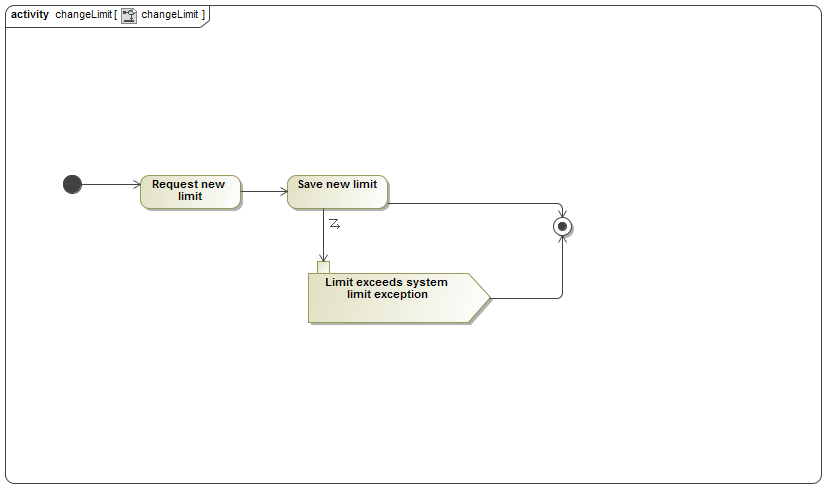
\includegraphics[width=1.0\textwidth]{images/changeLimit.png}
    \caption{setLimit activity diagram} 
\end{figure}

\begin{figure}[H]
	\centering
	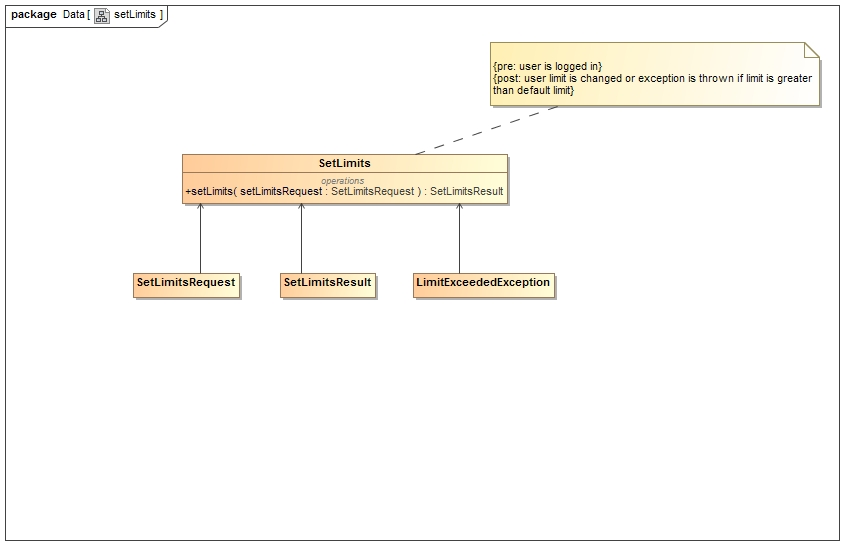
\includegraphics[width=1.0\textwidth]{images/setLimitsSC.jpg}
	\caption{setLimit service contract}
\end{figure}

%% -------------- REQUIRED FUNCTIONALITY --------------------
\subsection{Required Functionality}

%% --------------PROSESS SPECIFICATION ------------------------
\subsection{Process Specification}
 
%%--------------- DOMAIN MODEL ---------------------------------
\subsection{Domain Model}


\section{Open Issues}








\end{document}

